Having all above, assume we have initial semantic version of our application as \texttt{v1.0.0},
so that we must release upcoming version.
The version \texttt{v1.0.0} has been tested by QA team, so that release was approved by whole team.
General release steps to perform are following
\begin{enumerate}
    \item \textbf{Code phase.}
    Software engineer creates pull request from recent \texttt{feature} branch to \texttt{master} branch,
    this pull request triggers Continuous Integration (CI) to start, CI runs tests, code quality checks etc.,
    but deployment is not started yet, only CI\@.
    \item \textbf{Code phase.}
    After all CI checks passed, pull request reviewed by team and every comment from code review is fixed --
    the \texttt{feature} branch is ready to be merged into \texttt{master} branch.
    No CI/CD pipeline triggered by the merge.
    \item \textbf{Code phase.}
    Next, release engineer reviews software product changes documenting them in \texttt{CHANGELOG} file.
    Release engineer decides on the next Semantic Version~\cite{SemanticVersioning} increment.
    For example, software product has breaking changes,
    then release engineer decides to increment the major part of semantic version, so that \texttt{v0.1.1 -> v1.0.0}
    \item \textbf{Code phase.}
    Release engineer creates new release as follows
    \begin{itemize}
        \item Checkout to release branch: \texttt{git checkout -b release/v1.0.0}
        \item Adding minor changes and \texttt{CHANGELOG} file update
        \item Push release branch to remote: \texttt{git push origin release/v1.0.0}
        \item Create tag: \texttt{git tag -a v1.0.0 -m "Release v1.0.0"}
        \item Push tag: \texttt{git push origin v1.0.0}
    \end{itemize}
    \item \textbf{Build phase.}
    When new \texttt{TAG} is pushed to the remote repository, the build pipeline is being triggered~\cite{AzurePipelinesTriggers},
    initializing the build phase of DevOps cycle.
    Therefore, the code is being built, tested and specific artifacts are being created and published.
    \item \textbf{Release phase.} Release engineer validates the build artifacts,
    underlying infrastructure and deployment automations, ensuring smooth and reliable upcoming deployment.
    \item \textbf{Deploy phase.}
    There are a few deployments scheduled including the environments \texttt{DEV}, \texttt{QA}, \texttt{UAT}.
    Deployments to \texttt{QA} and \texttt{UAT} environments are to be approved by designated personnel,
    meanwhile \texttt{DEV} environment to be deployed automatically.
    \item Finally, the \texttt{Release/v*} branch is merged back to \texttt{master} after deployment is complete.
\end{enumerate}
Entire release process is shown on the picture below
\begin{figure}[H]
    \centering
    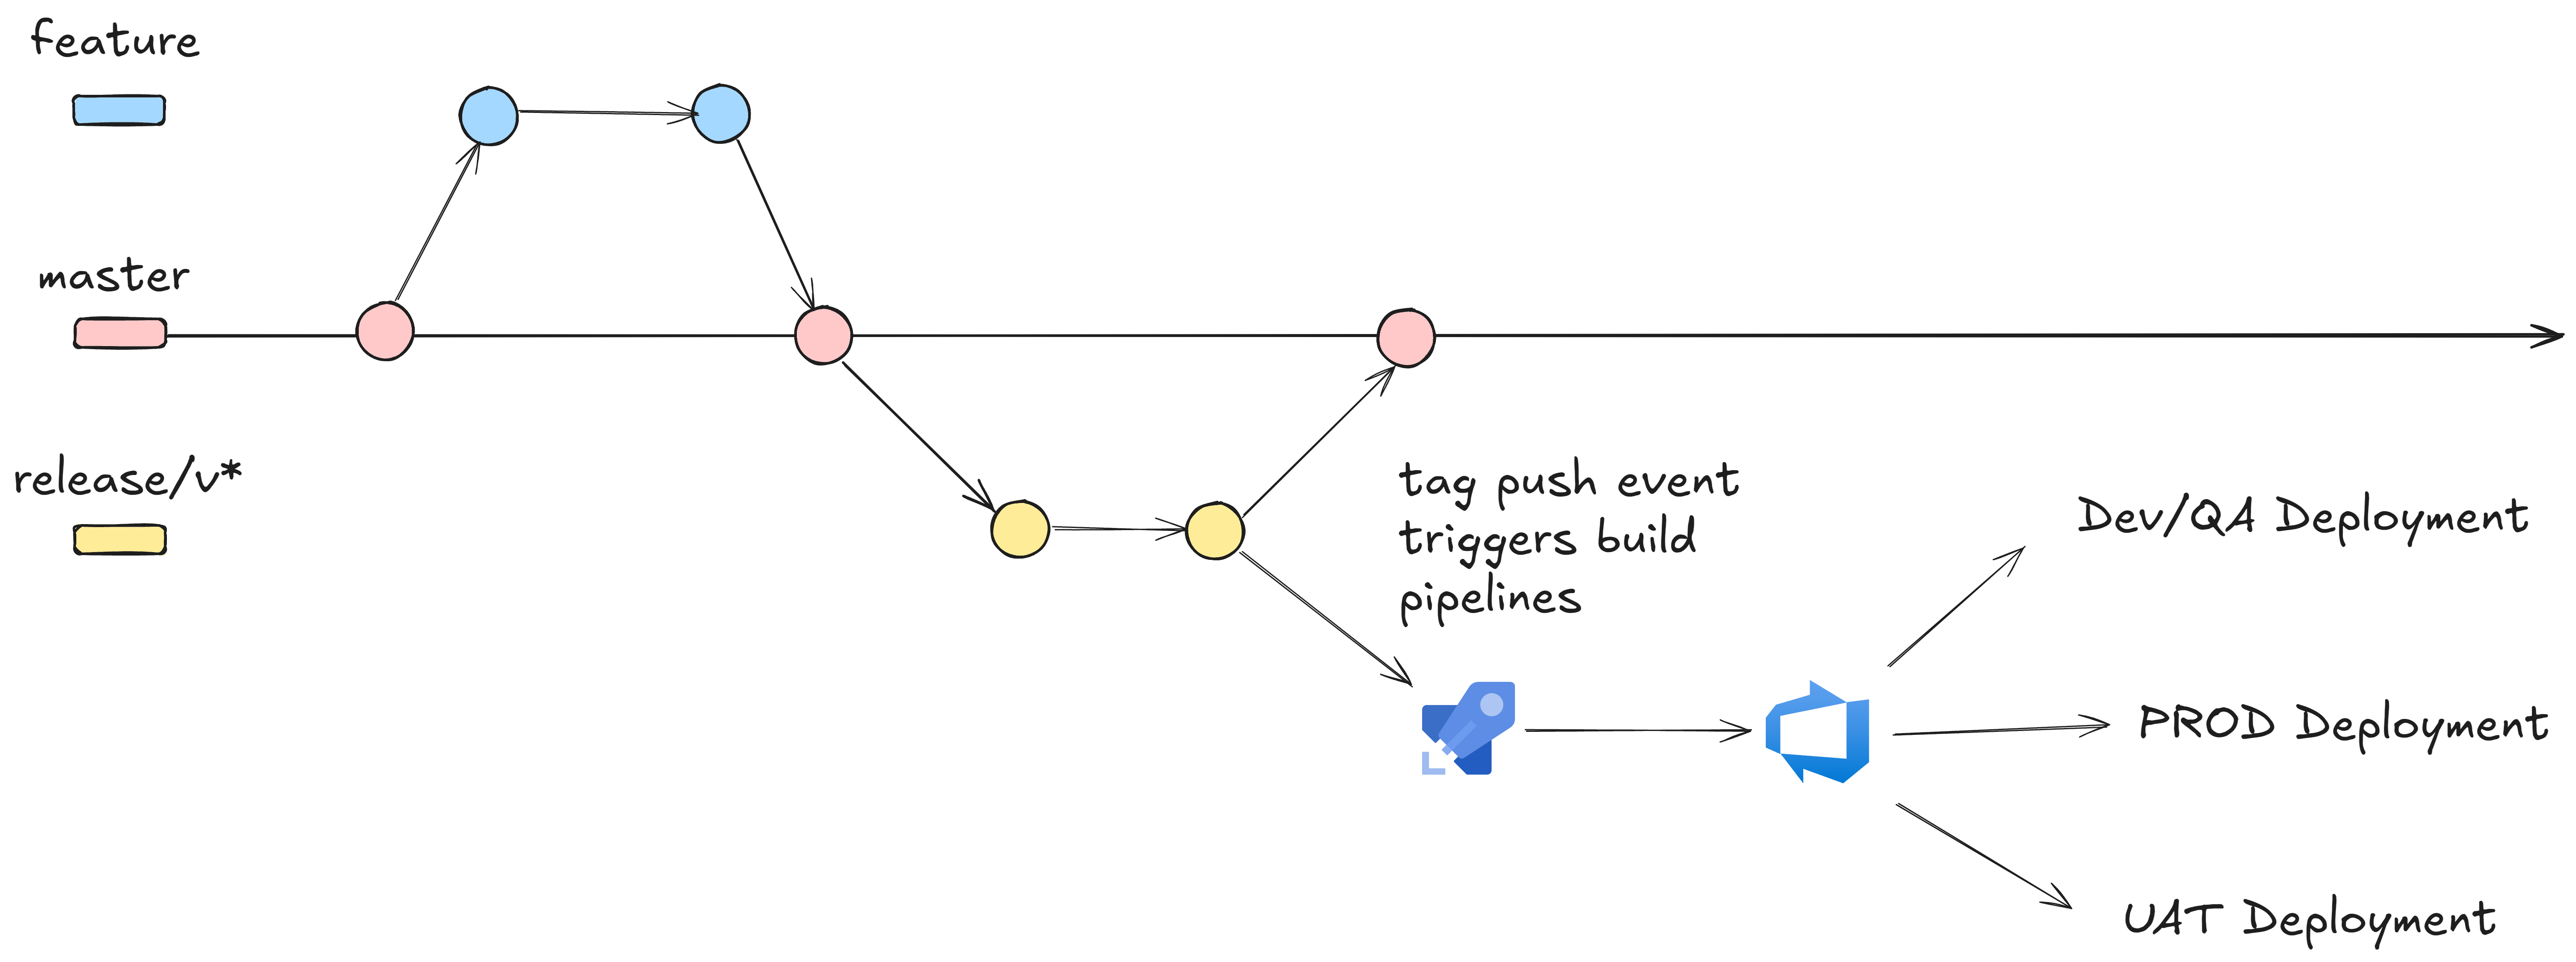
\includegraphics[width=1\textwidth]{img/Release_Flow}
    ~\caption{Release flow diagram.}\label{fig:gitlab-flow}
\end{figure}

